\documentclass{article}
\usepackage{amsmath}
\usepackage{amsfonts}
\usepackage{amssymb}
\usepackage{mathrsfs}
\usepackage{cancel}

\usepackage{graphicx}


\setlength\parindent{0pt}

\author{Pranav Tikkawar}
\title{TODO}

\begin{document}
\maketitle

\section{Section 1}
\begin{figure}[ht]
    \centering
    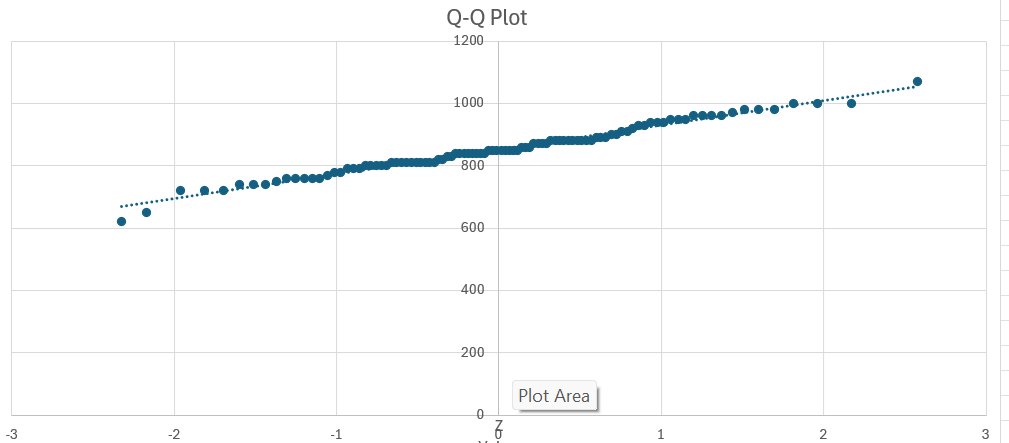
\includegraphics[width=0.8\textwidth]{A4IMG/QQPlot.png}
    \caption{QQ Plot}
    \label{fig:qqplot}
\end{figure}

\section{Section 2}
% Is it plausible to conclude the 100 times recorded follow a normal distribution
% approximately? Justify your answer
The QQ plot above looks relatively linear and the points are close to the line. This suggests that the data is normally distributed. However, the tails of the QQ plot are not perfectly linear, which suggests that the data may not be perfectly normally distributed. Therefore, it is plausible to conclude that the 100 times recorded follow a normal distribution approximately.

\section{Section 3}
% Construct a two-sided 90% Confidence Interval for the standard deviation of the time
% measurement for the device being evaluated in the dataset?
The 90\% confidence interval for the standard deviation of the time measurement for the device being evaluated in the dataset is $(70.82, 89.56)$. This was calculated using the formula:
\begin{align*}
    \left(\sqrt\frac{(n-1)s^2}{\chi^2_{\alpha/2, n-1}}, \sqrt{\frac{(n-1)s^2}{\chi^2_{1-\alpha/2, n-1}}}\right)
\end{align*}
where $n = 100$, $s = 79.01$, and $\alpha = 0.1$.

\section{Section 4}
% Sarpeidon Incorporated’s internal calibration standards requires the tester perform the
% following hypothesis test for each Atavachron produced,
% H0: σ = 80 nanoseconds vs. HA σ ≠ 80 at level of significance α0 = 0.1.
% If a device is produced that rejects this null hypothesis based on the results of the
% calibration testing, the device is deemed ineligible for sale. For the device being tested
% in the dataset, would Mr. Atoz approve the device for sale?

The null hypothesis is $H_0: \sigma = 80$ nanoseconds and the alternative hypothesis is $H_A: \sigma \neq 80$ nanoseconds. The level of significance is $\alpha = 0.1$. The test statistic is calculated as:
\begin{align*}
    \frac{(n-1)s^2}{\sigma^2} = \frac{99 \cdot 79.01^2}{80^2} = 96.57
\end{align*}
The critical values for the test statistic are $\chi^2_{0.05, 99} = 123.22$ and $\chi^2_{0.95, 99} = 77.05$. Since the test statistic is in between the critical values, we fail to reject the null hypothesis. Therefore, Mr. Atoz would approve the device for sale.



\end{document}